\section{系统设计}

\subsection{系统总体框图}

系统总体框图如\xref{fig:系统总体框图}所示,以安路科技EG4S20BG256的FPGA芯片为中心
\begin{itemize}
    \item 显示屏:实现画面输出,分辨率$1024\times 600$,使用HDMI进行连接。
    \item 扬声器:实现音频输出,可以控制音符的长度和音高,使用3.5mm音频接口。
    \item WII手柄:实现体感控制,具有加速度传感器和若干按钮,使用IIC协议。
    \item 键盘:实现按键输入,具有$4\times 4$共16个按键。
    \item 七段数码管:共$4$个,用于数字显示。
    \item 发光二极管:共$8$个,用于系统调试。
    \item 开关:共$8$个,用于系统调试。
\end{itemize}

\begin{Figure}[系统总体框图]
    
\includegraphics{build/Section01_01.fig.pdf}
\end{Figure}

\subsection{系统总体架构}
系统总体架构如\xref{fig:系统总体架构}所示,自底向上可以分为硬件电路层、硬件抽象层、软件逻辑层三个层次。硬件电路层和硬件抽象层构成了硬件部分。硬件电路层使用Verilog语言在FPGA上实现所需的硬件模块或物理硬件的驱动模块,将硬件的行为与寄存器中的数值相关联,并搭载Arm Cortex M0软核处理器。硬件抽象层则使用C语言将相关硬件的寄存器封装为C语言可操作的对象,并在此基础上,编写一些函数使软硬件之间的交互更为便利。软件逻辑层则构成软件部分,其实现了游戏的主体内容,这主要包括游戏本身的玩法和交互逻辑、游戏各界面的具体显示内容、游戏各界面间的切换等。

\begin{Figure}[系统总体架构]
    \includegraphics{build/Section01_02.fig.pdf}
\end{Figure}

\subsection{系统软硬件功能划分}
系统的软硬件功能划分如下:硬件部分负责实现诸如显示编码、数码管扫描、蜂鸣器驱动等对速度要求较高,需要复杂时序控制的部分。硬件部分将外设封装为若干寄存器,使得软件部分不需要关心驱动外设所需的时序,而是可以直接通过寄存器操作外设的工作状态。软件部分负责游戏功能的实现,根据输入和游戏逻辑控制图像和声音。

\subsection{系统构成}
系统硬件主要由三部分组成:硬木课堂EG4S20核心板、自制的扩展板、自制的产品外壳。如\xref{fig:系统硬件构成}所示,其中黑色的是硬木课堂的核心板,其下绿色的是自制扩展板。

系统需要连接三个外设
\begin{enumerate}
    \item 通过HDMI接口连接显示屏。
    \item 通过3.5mm音频接口连接扬声器。
    \item 通过WII手柄接口连接WII Nunchunk手柄。
\end{enumerate}

\begin{Figure}[系统硬件构成]
    \includegraphics[width=10cm]{image/4.pdf}
\end{Figure}

\subsubsection{自制扩展板}
自制的扩展板通过KiCad 7.0软件进行设计,由嘉立创生产,其取代了原先硬木课堂扩展板的即有功能,并根据项目需要,实现了若干新功能,同时,通过合理排布插排位置,使扩展板可以置于核心板的正下方,减小了电路板的实际占用空间,为产品外壳的设计提供了可能。自制扩展板的原理图与版图,如\xref{fig:自制扩展板}所示,其主要实现了以下功能
\begin{itemize}
    \item USB Type C输入。其连接至板上USB HUB控制器芯片CH334U,分别接至四处。两处是位于扩展板中央的两个Type A接口,其通过软硅胶线,分别连接至核心板的硬件烧写和串口通讯接口。一处是位于扩展板左侧的Type A接口,其用于向显示屏和扬声器供电。一处是通过板内连线接至板上的调试器。由此,系统调试中“硬件烧写、软件调试、串口通讯”仅需要一根Type C线即可实现,不再需要分别准备三根Micro B线。同时,系统可以直接向显示屏和扬声器供电。
    \item HDMI接口。显示输出,将核心板产生的HDMI信号输出至显示屏。
    \item 3.5mm接口。音频输出,将核心板产生的用于驱动蜂鸣器的信号输出至外置扬声器。扩展板上设计了一阶RC低通滤波电路,滤除高次谐波以提高声音质量。
    \item WII接口。依据WII Nunchunk手柄的接口,在扩展板板边制作了相应的边缘连接器(金手指),使得手柄可直接连接在电路板上,不再需要使用杜邦线连接。
\end{itemize}

\begin{Figure}[自制扩展板]
    \begin{FigureSub}[原理图]
        \includegraphics[width=14cm]{image/Adapter.pdf}
    \end{FigureSub}\\ \vspace{0.5cm}
    \begin{FigureSub}[版图]
        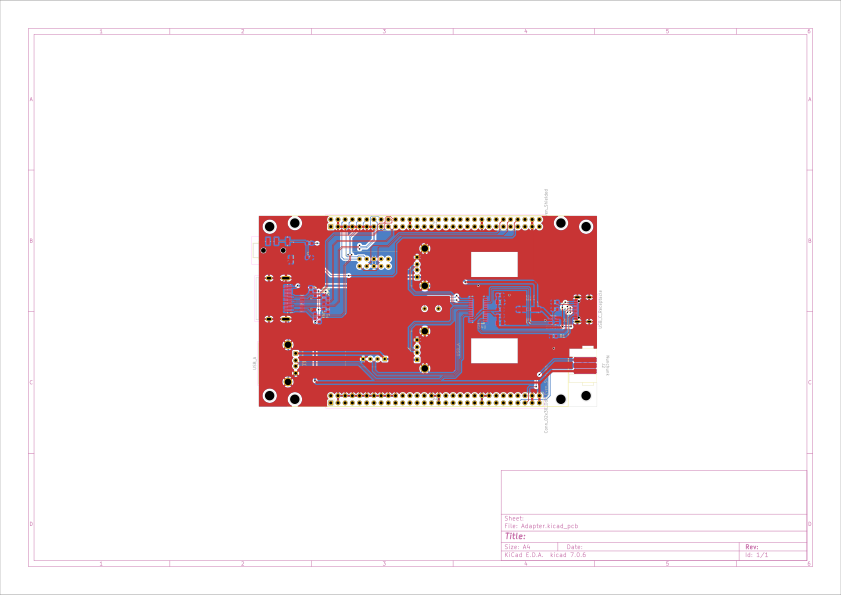
\includegraphics[width=14cm]{image/Adapter_PCB.pdf}
    \end{FigureSub}
\end{Figure}

\subsubsection{自制产品外壳}
产品外壳通过Inventor软件设计,由嘉立创生产。产品外壳分为主体和上盖两部分。外壳主体如\xref{fig:外壳主体}所示,通过铝合金CNC加工,表面阳极氧化处理。外壳主体内放置电路板,通过螺丝固定。外壳主体侧边开槽,用于外部连接电路板边沿的相关端口。外壳上盖如\xref{fig:外壳上盖}所示,材质为透明亚克力,透过上盖可以看到其下的电路板。

产品外壳简洁美观,其使游戏机不再是一块裸露的电路板,而更接近于实用产品。


\begin{Figure}[自制产品外壳]
    \begin{FigureSub}[外壳主体]
        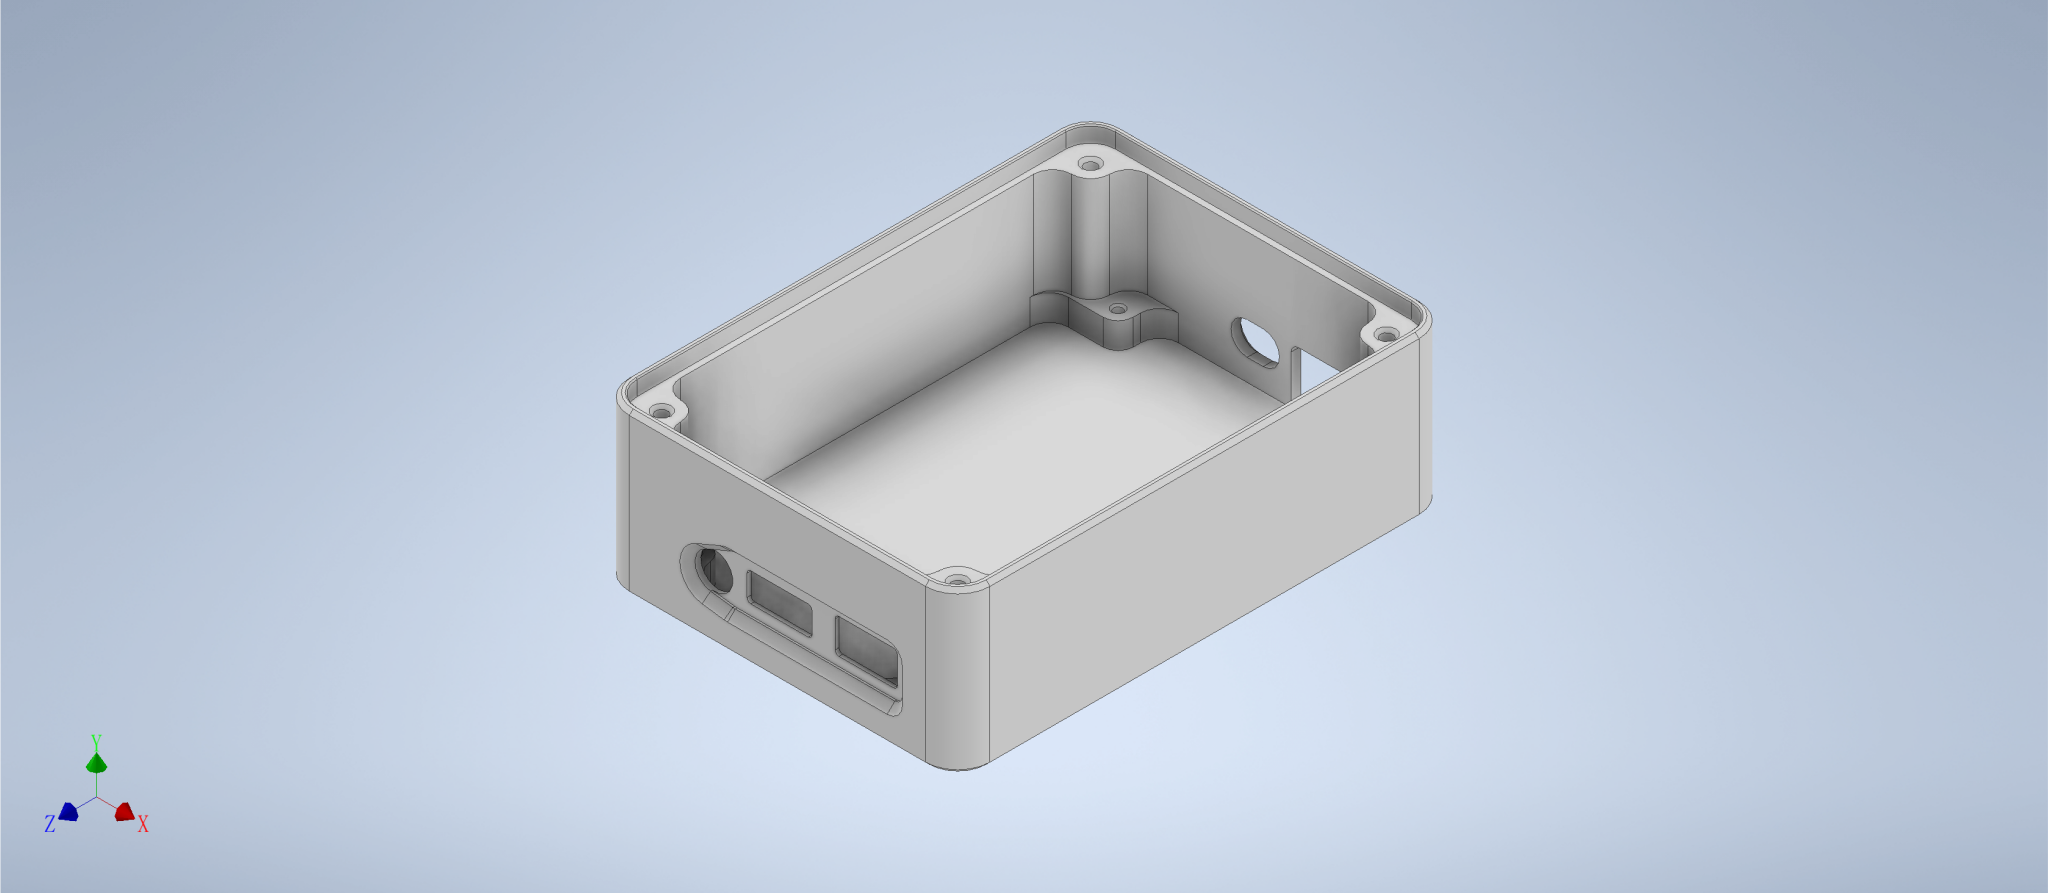
\includegraphics[width=15cm]{image/PrismGCNew_3D.pdf}
    \end{FigureSub}\\ \vspace{0.5cm}
    \begin{FigureSub}[外壳上盖]
        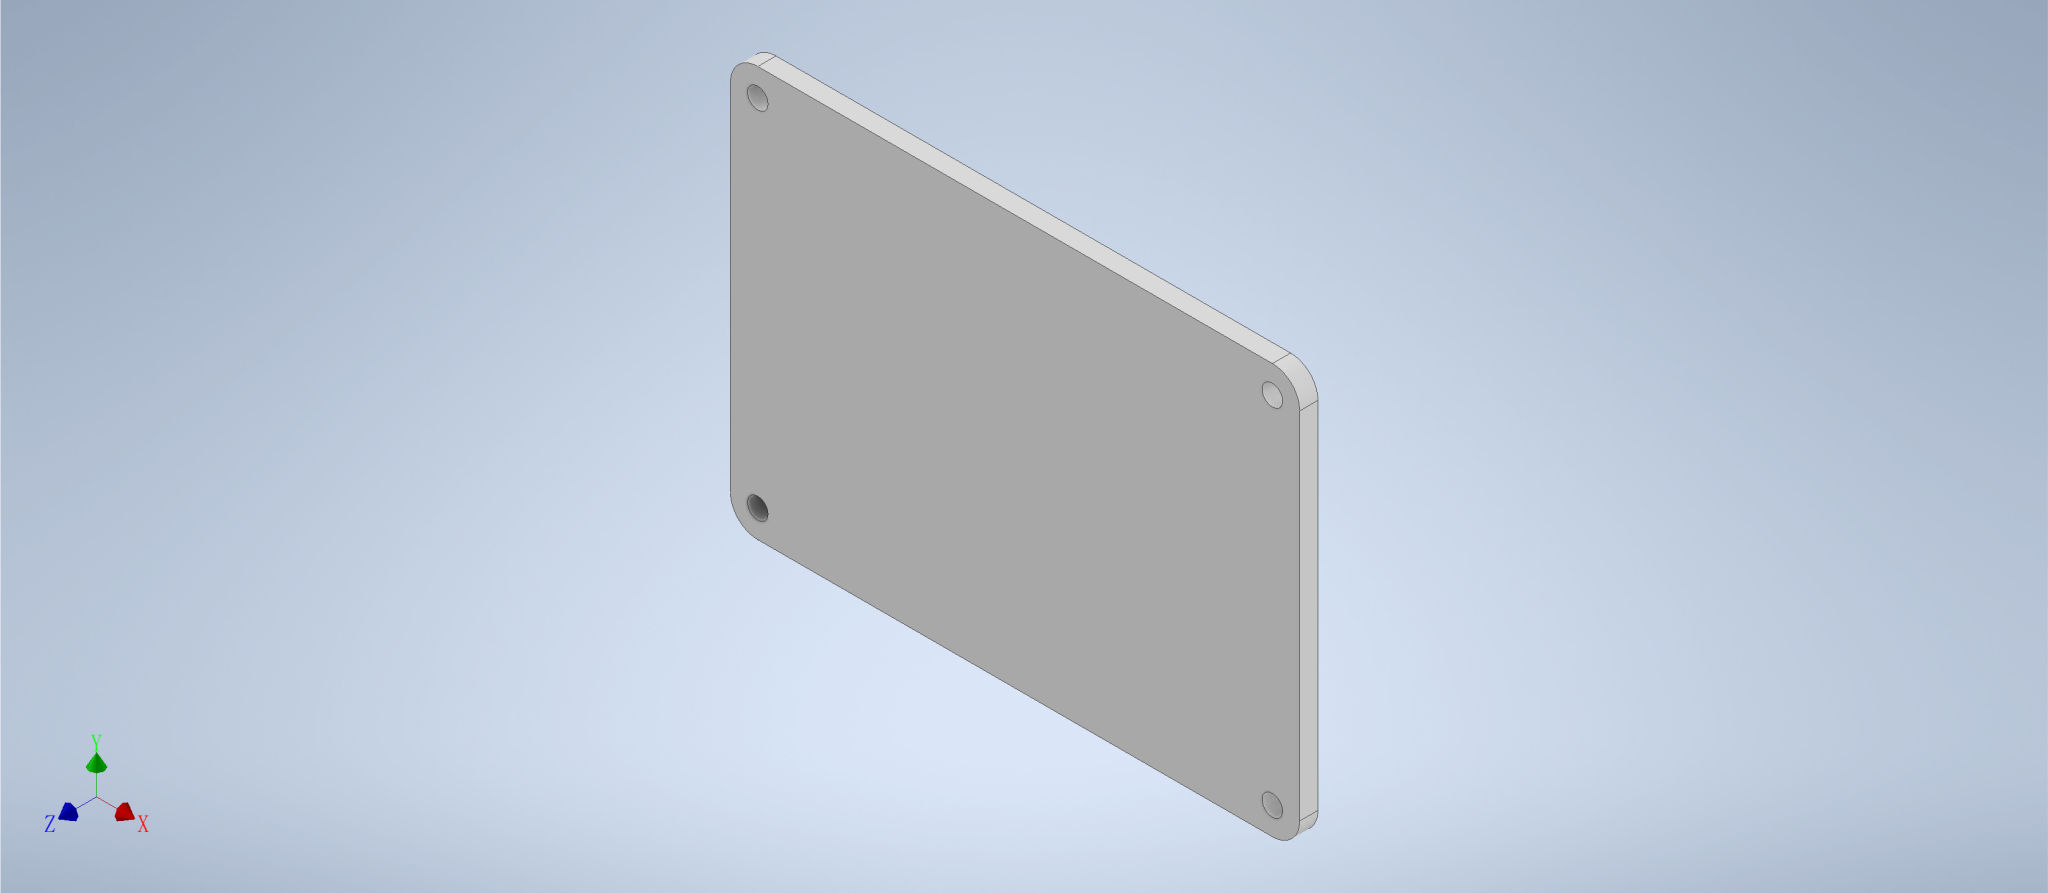
\includegraphics[width=15cm]{image/002_3D.pdf}
    \end{FigureSub}
\end{Figure}


\subsection{系统完成进度}
系统至决赛以完成其预定设计目标,作为游戏机具备可玩性和产品性。

显示部分,初赛时已经成功地在FPGA上实现了HDMI协议,可以点亮屏幕。并且成功地利用了FPGA片上的SDRAM资源作为显存,可以实现Cortex M0对显示屏的单像素控制。同时在显存使用上应用了双缓存机制,避免了显示刷新过程中的闪烁问题。复赛期间通过改进硬件和软件,大幅度提高了显示效率,使得丰富的游戏画面和内容成为可能性。同时,实现了字符显示,基于$8\times 16$点阵字体,支持成倍缩放,支持格式化字符串显示输出。类似技术,也被应用于实现特定图案(例如游戏主角)的显示。决赛期间进一步优化显示,硬件上取消了写入部分的FIFO,使显示数据写入直通显存,进一步提高了显示效率和可靠性,将游戏画面的帧时长控制在$150\si{ms}$内(普遍在$100\si{ms}$至$120\si{ms}$间)。软件底层在写显存前进行了若干预处理,解决了过去复赛期间由于片上SDRAM自身硬件特性导致的若干显示故障和异常,显示体验显著改善。

音频部分,目前可以利用自制扩展板上的3.5mm音频接口连接外置扬声器,或使用板载蜂鸣器,发出特定音高和音长的音符。在Cortex M0的控制下,可以根据游戏进程播放不同的提示音,丰富游戏交互体验。同时,也可以播放简单的背景音乐。

输入部分,初赛期间WII手柄已在Arduino平台上完成功能测试,尝试将与WII手柄交互所用的IIC协议在FPGA上硬件实现但未完成。复赛期间在IIC协议的硬件实现上遇到了较大的阻力和困难,故随即改变方案为软件实现,具体而言,即将所需的两路信号SCL和SDA挂载于GPIO,随后通过软件来实现IIC协议所需的时序。复赛期间WII手柄已经成功接入系统中,系统可以获得手柄的摇杆或手柄的加速度传感器的数据,通过摇杆或体感进行控制,实现智能化交互。决赛期间,在自制扩展板上设置了WII手柄的接口,WII手柄可以直接连接在板子上,不再需要通过杜邦线连接。

游戏部分,初赛期间曾以一个极简单的游戏“别踩黑线”作为系统的验证。复赛期间,则重新设计了一款全新的游戏“无敌史莱姆大冒险”。游戏具有明确独特的核心玩法和丰富的关卡,且具备相当的可玩性。决赛期间进一步扩展游戏关卡和游戏元素,并将游戏的软件程序固化到硬件中,游戏机上电就能开始工作,不再需要连接调试器。
